\documentclass[a4paper,12pt,oneside]{scrreprt}
\usepackage[latin1]{inputenc}
\usepackage[T1]{fontenc}
\usepackage{ae,aecompl}
\usepackage[english]{babel}
\usepackage{amsmath}
\usepackage{amssymb}
\usepackage{amsfonts}
\usepackage{amsthm}
\usepackage{graphicx}
\usepackage{wrapfig}
\usepackage{ulem}
\usepackage{cancel}
\usepackage{float}
\usepackage{color}
\usepackage{titlesec}
\usepackage{geometry}
\geometry{verbose,a4paper,tmargin=25mm,bmargin=25mm,lmargin=15mm,rmargin=25mm}
\titlelabel{\thetitle.\quad}
\usepackage{tabularx}
\usepackage{booktabs}
\usepackage{paralist}
\usepackage{textcomp}

\renewcommand{\rmdefault}{phv}
\renewcommand{\sfdefault}{phv}

\usepackage{listings}
\lstset{
	% numbers=left,
	breaklines=true,
	tabsize=2,
	literate={\ \ }{{\ }}1,
	%	language=C,
	basicstyle=\footnotesize\ttfamily, 
	stepnumber=1,
	%	aboveskip=-10pt,
}


\begin{document}
\begin{tabular}{ccc}
	\begin{large} \textbf{Prof. Lichter} \end{large} &
	
	\begin{minipage}[H]{3.5cm}
	\centering
		\begin{large} OOSC \end{large} \\
		\begin{large} WS 2016/2017 \end{large}
	\end{minipage} &
	
	\begin{minipage}[H]{4cm}
%		\includegraphics[keepaspectratio,width=\textwidth,angle=0]{logoswc.png}
	\end{minipage} \\
Andreas Steffens, Konrad F\"ogen &  &  \\
& \begin{huge} \textbf{Submission 1} \end{huge}&  \\
& oosc@swc.rwth-aachen.de &  \\
& & \\
 % Hier drunter müssen die Daten noch angepasst werden
Issued: 1.1.2016 &
Submission: 1.1.2016 &
Discussion: 1.1.2016 \\
\end{tabular}
\newline \newline \newline

\begin{center}
	Submitted by Group 09
	
	\bigskip
	
	\begin{tabular}{ll}
		Ulfet CETIN & 391819 \\
		Saud KHAN & 392365  \\
		Samuel ROY & 391822 \\
		Charulekha, Besta Venkateswara RAO & 391844 \\
		Deepak SATEESH & 391813  \\
	\end{tabular}
	
	(ordered on lastname basis)
	
\end{center}


\setcounter{chapter}{1} % Aktuelles Assigment
	
\section{Task: Develop a Metric for "Readability"}

	\begin{enumerate}[a)]
		\item Develop a calculated, precise metric (cf. with lecture slides) for readability of code on
method-level. The goal of the metric is to indicate how easy / fast it is to get the intent of a
method.
		
			\textbf{Constructive Metric Development}:
			\begin{enumerate}[1)]
				\item Identify a relevant quality aspect:\\
				readability of code on method-level\\
				
				
				\item Model the relevant quality aspect:\\
				readability of code on method-level:\\
				methods that have Java documentation comment,
				and those who do not
				
				Information:\\
				Java document comment (official form) has the following structure, which we will use to generate our metric:
				
				\begin{addmargin}[-2em]{2em}
					\begin{lstlisting}
					/**
						some comment about the method
					*/
					\end{lstlisting}
				\end{addmargin}
				
				
				\item Determining a scale:\\
				readability of code on method-level:\\
				a real number r in range [0,1]
				
				\item Develop the metric calculation\\
				readability of code on method-level:\\
				relation between all the methods that have Java document comment and the all the methods that is there in the code
				
				\item Develop measurements\\
				readability of code on method-level:\\
				methods (and their respective Java document comments (if any))
				
				\item Apply and improve the metric:\\
				Code Readability on Method-Level:\\
				
				$ codeReadability =  \dfrac{number\_of\_methods\_that\_have\_JavaDocStyle\_comments}{number\_of\_all\_methods}$
				
				
			\end{enumerate}
			
		
		\item Evaluate your metric by applying it to the example code and discuss the evaluation.
		
		Metric should be interpreted as follows:
		\begin{itemize}
			\item All the Java source has to be traversed and functions has to be counted:
				\begin{itemize}		
					\item all the methods that have Java documentation comment
					\item all the methods (irrespective of whether they have Java documentation or not)
				\end{itemize}
			\item ( alternatively, javadoc command of javac can be used to generate a documentation information that gives out which functions have a Java documentation comments )
				\begin{itemize}
					\item Item.java:
					
						\begin{tabular}{|l|l|l|}
							\hline
							1) & Item(final String value, final Item next) {...} & - no comment\\
							2) &public Item next() {...} & - no comment\\
							3) &public String value() {...} & - no comment \\
							\hline
						\end{tabular}
					
					\item	List.java:
					
						\begin{tabular}{|l|l|l|}
							\hline
							
							4) & private List(final Item head)  & - no comment\\
							
							5) & public static List of(final String... values)  & - no comment\\
							
							6) & public boolean containsValue( &	- has "Java document comment" \\
							
							& \hspace{1em}final String value, final int itemLimit) & \hspace{1em}formatted comment\\
							
							7) & private Predicate<Item>  & - no comment\\
							& \hspace{1em} itemValueEqualsTo(final String value) & \\
							8) & private Stream<Item> itemsStream() & - no comment\\
							9) & public String toString() & - no comment\\
							10) & private boolean endOfList(Item node) & - no comment\\
							\hline
						\end{tabular}
				\end{itemize}
		\end{itemize}
		\bigskip
		
		The only Java documentation comment that is there in the given code, for demonstration purposes:
		\begin{addmargin}[1em]{2em}
			\begin{lstlisting}
			/**
			* Search through the list for given value while considering only itemLimit.
			*
			* @param value search value
			* @param itemLimit number of items to consider
			* @return true, if value is in peek of this list
			*/
			\end{lstlisting}
		\end{addmargin}
		
		
		
		
		
		$ codeReadability =  \dfrac{number\_of\_methods\_that\_have\_JavaDocStyle\_comments}{number\_of\_all\_methods}$
		
		$number\_of\_methods\_that\_have\_JavaDocStyle\_comments = 1$
		
		$number\_of\_all\_methods = 9$
		
	\end{enumerate}

\clearpage
	
\section{Task: Develop a Quality Model for Theses}

Develop a quality model for bachelor- and master theses. Dimensions which should be included in the quality model are a) process and working behavior, b) thesis report and, c) source code artefacts.

	\begin{enumerate}[a)]
		\item Develop at least two characteristics for each dimension and explain each one of them in a few sentences.
			\begin{enumerate}[a)]
				\item process and working behaviour
					\begin{itemize}
						\item Methodology: \\
						Aims to evaluate an investigation of a research problem and the reasoning for the application of specific procedures or techniques used to identify, select, process, and analyze information applied to understanding the problem. 
						
						\item Literature Analysis:\\
						An academic work requires detailed analysis of literature. This characteristic aims to analyze if the author has not only cited the sources but also adapt and reflect on them critically.
					\end{itemize}
				
				\item b) thesis report
				\begin{itemize}
					\item Content:\\
					The content should be a discussion on the research question which is assessed in terms of relevance to solution of the objective and depth and criteria of consistency. 
					
					\item Form and style:\\
					The formal requirements for this characteristic would be page size, justification, proportional script (text: Times New Roman, titles: Arial), font size, line spacing,  paragraphs are to be separated by blank lines , headers and footers, margins etc.
				\end{itemize}
			
				\item c) source code artefact
				\begin{itemize}
					\item Usability: \\
					Here it refers how the source code can easily be used and installed. It also refers to methods for improving ease-of-use of code during the process.
					
					\item Coding Standards:\\
					A�coding standard�lists several�rules to be followed during�coding, such    as the way variables are to be named, the way the code is to be laid out, error return conventions, etc.    
				\end{itemize}
			\end{enumerate}
		
		\item Develop at least three sub-characteristics for each characteristic and explain each one of them in a few sentences. You don?t need to specify any metrics!
			\begin{itemize}[-]
				\item Methodology: 
					\begin{enumerate}[1.]
						\item Appropriateness: \\
						Appropriateness can mean tailoring the process being used in the thesis. The methods or procedures being used can be in a qualitative way. The argumentation and the choice of adequate research methods.
						
						\item Validity: \\
						Validity of research can be explained as an extent at which requirements of scientific research method have been followed during the process of generating research findings within an appropriate time scale.
						
						\item Reliability: \\
						Reliability refers to the extent to which the same results can be obtained using the same instruments more than one time. In simple terms, if a research is associated with high levels of reliability, then other researchers need to be able to generate the same results, using the same research methods under similar conditions.
					\end{enumerate}
				
				\item Literature Analysis:
					\begin{enumerate}[1.]
						\item Depth of Analysis:\\
						 An academic paper requires an extensive and detailed analysis of literature. It is essential to not only analyse general basic literature (textbooks) but also special literature on the respective topic.
						
						\item Quality:\\
						 The author should reflect on the basic quality criteria of scientific research (validity, reliability, representativeness, etc.) and demonstrate how they were taken into consideration. Other criteria are the topicality and range of used literature
						
						\item Transparency of references: \\
						Transparency�in�reporting of research is essential for providing enough information about how the work was performed to allow others to replicate it. In a thesis paper, all explanations that have been adopted literally or analogously have to be marked as such.
					\end{enumerate}
				
				
				
				
				\item Content:
				\begin{enumerate}[1.]
					\item Consistency of argumentation: \\
					In academic writing, an�argument�is usually a main idea, often called a "claim" or "thesis�statement", backed up with evidence that supports the idea. Consistency should be there �in the title, problem, purpose, and research question improve the logic and transparency�.
					
					\item Originality: \\
					Originality�in research mean what you are doing is from your own perspective although you may draw arguments from other research work to back up your arguments.
					
					\item Contribution to knowledge: \\
					Contribution to knowledge�means creating new�knowledge�based on the previously available�knowledge�by doing extensive and innovative�research.
				\end{enumerate}
				
				
				
				
				
				\item Form and style:
				\begin{enumerate}[1.]
					\item Precision:\\
					 It refers to the extent of adherence to the prescribed format. More the adherence more the Precision.
					
					\item Illustration through figures and tables:\\
					 How many sections are using figures and tables to explain the underlying concepts and their examples.  
					
					\item Correctness: \\
					How correct are the facts and figures mentioned in the report.
				\end{enumerate}
				
				\clearpage
				
				\item Usability:
				\begin{enumerate}[1.]
					\item Learnability:\\
					describes the ability of an interface to allow users to accomplish tasks on the first attempt. A more learnable system is one that reduces the time it takes to complete the tasks as users spend more time with the system faster than others.
					
					\item Understandability: \\
					How easy is it to understand the code. Not so complex code is easier to understand and comment also help in the understandability. 
					
					\item Operability: \\
					How easy is to install and run the code .Also how intuitive or guided the flow is. 
				\end{enumerate}
				
				
				
				\item Coding standards:
				\begin{enumerate}[1.]
					\item Comments: \\
					Comments can be helpful to understand the intent or the motive of the method if the code is complex or unreadable. It also helps the non-coder to understand what that method does.
					
					\item Naming conventions: \\
					It helps to relate similar entities and gives the user a broader picture.
					
					\item Error Handling: \\
					This is most useful for debugging and preventing the system crash.
				\end{enumerate}
				
				
			\end{itemize}
		
		\item Visualize your model in an appropriate form.
			\begin{figure}[H]
				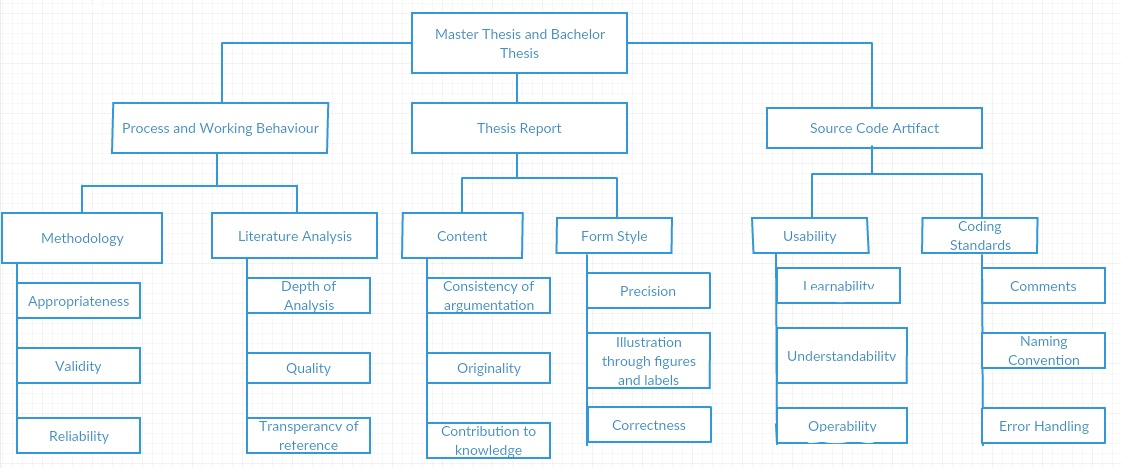
\includegraphics[scale=0.45]{graph.jpg}
			\end{figure}
		
		\item Propose an aggregation formula for the overall assessment based on the
		(sub-)characteristics of your quality model. The overall assessment should result in a
		grade from 1.0 to 5.0. Explain and justify your proposal.
		
		The scoring used here is a non- weighted scoring (giving equal importance to Process and Working Behavior, Thesis Report, and Source Code Artifacts) as we are normalizing the total score in the end using the formula below. The metric has different scoring ranges so that the examiner can evaluate each metric in a different way, for example "Validity" metric for Methodology can only be either "the Methodology used in thesis is valid", or "Methodology used in thesis is invalid", so scoring is  0-1. For another example the "Quality Metric" in Literature Analysis, the scoring is between 0-10, ranging from "lacks quality" to "High quality".\\
		
		\begin{center}
			
		$a_i = \dfrac{a_i - min(a)}{max(a) - min(a)} * (high-low) + low$
		\end{center}
				
		\item Implement your Quality Model as a Spreadsheet (Excel/OpenOffice).\\
			The respective file could be find in the submission archive we sent.
	\end{enumerate}

	

\end{document}
